% -----------------------------------------------------------------------
% Template Skripsi untuk MIPA
% 
% @author Yusuf Syaifudin
% @created 29/02/2016
% 
% -----------------------------------------------------------------------

\documentclass[ugmtesis]{ugmtesis}

% ------------------------------------------------------------------------------
% Berisi tambahan package dan konfigurasi untuk masing-masing package.
% Ada baiknya, setiap konfigurasi diletakkan tepat dibawah 
% setelah package dilakukan import (usepackage) agar tidak membingungkan.
% Serta disarankan untuk menambah kegunaan package tersebut agar tidak lupa.
% ------------------------------------------------------------------------------


% font tambahan
\usepackage{textcomp}
\usepackage{amsfonts}

% digunakan untuk membuat flowchart
\usepackage{tikz}
\usetikzlibrary{shapes,arrows, fit, positioning}

\usepackage{float}
\usepackage{booktabs}
\usepackage{pbox}
\usepackage{multirow}
\usepackage[normalem]{ulem}
\useunder{\uline}{\ul}{}

% Untuk hyperlink dan otomatis membuat bookmark
\usepackage{hyperref}

% break tanda /, - dan spasi ke baris baru jika sudah tidak muat
\def\UrlBreaks{\do\/\do-\do\ }

% font url dibuat miring dan dg jenis font ttfamily
\renewcommand{\UrlFont}{\small\ttfamily\itshape}

\usepackage{csquotes}
\usepackage{framed}
\usepackage{enumitem}

% untuk input kode baik dari file atau bukan
\usepackage{listings} 
\usepackage{xcolor}

% ----------------------------------------------------------------------------
% Contoh dari file
% ----------------------------------------------------------------------------
% \begin{figure}[H]
%   \lstinputlisting[language=python, firstline=38, lastline=59]{code/linkwalker.py}
%   \caption{Mendapatkan daftar tautan berita pada kompas.com}
%   \label{grab daftar berita kompas}
% \end{figure}
% ----------------------------------------------------------------------------
% 
% ----------------------------------------------------------------------------
% Contoh
% ----------------------------------------------------------------------------
% \begin{figure}
% 	\begin{lstlisting}[language=sql]
% 		update train_data_statement set data = replace(data, '“', '"');
% 		update train_data_statement set data = replace(data, '”', '"');
		
% 		update test_data_statement set data = replace(data, '“', '"');
% 		update test_data_statement set data = replace(data, '”', '"');
% 	\end{lstlisting}
% 	\caption{\textit{Query} SQL untuk melakukan perubahan karakter pada data}
% 	\label{kueri SQL untuk melakukan perubahan karakter pada data}
% \end{figure} 
% ------------------------------------------------------------------------------

\usepackage{color}
\usepackage{amsmath}
\usepackage{courier}
\usepackage[scaled=.75]{beramono}

%-----------------------------------------------------------------
% Setting syntax hightlighting
%-----------------------------------------------------------------
\definecolor{codegreen}{rgb}{0,0.6,0}
\definecolor{codegray}{rgb}{0.5,0.5,0.5}
\definecolor{codepurple}{rgb}{0.58,0,0.82}

\lstset{frame=tb,
  language=Python,
  aboveskip=2mm,
  belowskip=1mm,
  showstringspaces=false,
  columns=flexible,
  basicstyle  = \fontfamily{pcr}\fontsize{8pt}{8pt}\selectfont,
  numbersep=8pt,
  numbers=left,
	numberstyle=\tiny\color{codegray},
  keywordstyle=\color{magenta},
  commentstyle=\color{codegreen},
	stringstyle=\color{codepurple},
  breaklines=true,
  breakatwhitespace=true,
  tabsize=4
}

% Untuk menghilangkan titik-titik pada daftar isi

\usepackage[titles]{tocloft}
\renewcommand{\cftdot}{}

% Untuk membuat multi kolom
\usepackage{etoolbox,refcount}
\usepackage{multicol}

% Konfigurasi multi kolom
% bikin multi kolom
\newcounter{countitems}
\newcounter{nextitemizecount}
\newcommand{\setupcountitems}{%
  \stepcounter{nextitemizecount}%
  \setcounter{countitems}{0}%
  \preto\item{\stepcounter{countitems}}%
}
\makeatletter
\newcommand{\computecountitems}{%
  \edef\@currentlabel{\number\c@countitems}%
  \label{countitems@\number\numexpr\value{nextitemizecount}-1\relax}%
}
\newcommand{\nextitemizecount}{%
  \getrefnumber{countitems@\number\c@nextitemizecount}%
}
\newcommand{\previtemizecount}{%
  \getrefnumber{countitems@\number\numexpr\value{nextitemizecount}-1\relax}%
}
\makeatother    
\newenvironment{AutoMultiColItemize}{%
\ifnumcomp{\nextitemizecount}{>}{2}{\begin{multicols}{2}}{}%
\setupcountitems\begin{itemize}}%
{\end{itemize}%
\unskip\computecountitems\ifnumcomp{\previtemizecount}{>}{2}{\end{multicols}}{}}
%end bikin multi kolom

% ------------------------------------------------------------------------------
% Contoh sintaks:
% ------------------------------------------------------------------------------
% \begin{itemize}
%   \item \textit{Reporting verb} yang hadir sebelum entitas pada kutipan langsung:
%   \begin{AutoMultiColItemize}
% 	  \item tutur
% 	  \item kata
% 	  \item ujar
%   \end{AutoMultiColItemize}

%   \item \textit{Reporting verb} yang hadir setelah entitas pada kutipan langsung:
%   \begin{AutoMultiColItemize}
% 	  \item mengatakan
% 	  \item menjawab
%   \end{AutoMultiColItemize}
% \end{itemize}
% ------------------------------------------------------------------------------


% Setting list agar spasi antar list tidak terlalu banyak
\setlist{  
  listparindent=\parindent,
  parsep=0pt
}

% Agar tetap Justify tapi kata tidak dipisah sesuka hati (not hypenation but justified)
\tolerance=1
\emergencystretch=\maxdimen
\hyphenpenalty=10000
\hbadness=10000
\hyphenchar\font=-1
\sloppy

% Agar support longtable
% https://tex.stackexchange.com/questions/639452/create-long-table-in-latex
% need: varwidth, ninecolors
%%%% begin of required preamble
\usepackage{tabularray}
\usepackage{longtable}
\UseTblrLibrary{varwidth}
\DefTblrTemplate{contfoot-text}{default}{Bersambung di halaman selanjutnya}
\DefTblrTemplate{conthead-text}{default}{(Lanjutan)}


% Konfigurasi variable seperti judul dan lain sebagainya
\titleind{AUTENTIKASI MESIN KE MESIN BERBASIS RISIKO PADA KASUS FHIR \textit{(FAST HEALTH INTEROPERABILITY RESOURCES)} MENGGUNAKAN RANDOM FOREST}

\titleeng{RISK BASED MACHINE TO MACHINE AUTHENTICATION IN FHIR CASE \textit{(FAST HEALTH INTEROPERABILITY RESOURCES)} USING RANDOM FOREST}

\fullname{Damar Arba Pramuditya}

\idnum{22/501365/PPA/06386}

\examdate{17 Januari 2024}

\degree{Master of Computer Science}

\yearsubmit{2024}

\program{Magister Ilmu Komputer}

\headprogram{Azhari SN, Dr., MT}

\dept{Ilmu Komputer dan Elektronika}

\firstsupervisor{Arif Nurwidyantoro, S.Kom., M.Cs}

\firstexaminer{Mhd. Reza M.I Pulungan, M.Sc., Dr.-Ing}

\secondexaminer{Sigit Priyanta, S.Si., M.Kom}



\begin{document}

%-----------------------------------------------------------------
% Disini awal masukan untuk muka skripsi
%-----------------------------------------------------------------

% Cover
\cover

% Halaman judul
\titlepageind 

% Halaman Persetujuan
\approvalpage

% Halaman Pernyataan
\declarepage

% Halaman Persembahan
\acknowledment
\begin{flushright}
\Large\emph\cal{Karya ini ku persembahkan kepada \\
Ibu, Bapak, Kakak-kakakku, dan keponakanku tercinta
serta semua teman-teman seperjuangan di Ilmu Komputer Universitas Gadjah Mada}
\end{flushright}

%-----------------------------------------------------------------
% Disini akhir masukan untuk muka skripsi
%-----------------------------------------------------------------

% Motto
\input{BAB_TESIS/BAB0/2_MOTTO}

% Prakata
\input{BAB_TESIS/BAB0/3_PRAKATA}

%-----------------------------------------------------------------
% Daftar Isi
%-----------------------------------------------------------------
\newpage
\phantomsection
\addcontentsline{toc}{chapter}{\contentsname}
\tableofcontents
%-----------------------------------------------------------------
% Akhir Daftar Isi
%-----------------------------------------------------------------

%-----------------------------------------------------------------
% Daftar Tabel
%-----------------------------------------------------------------
\newpage
\phantomsection
\addcontentsline{toc}{chapter}{\listtablename}
\listoftables
%-----------------------------------------------------------------
% Akhir Daftar Tabel
%-----------------------------------------------------------------

%-----------------------------------------------------------------
% Daftar Gambar
%-----------------------------------------------------------------
\newpage
\phantomsection
\addcontentsline{toc}{chapter}{\listfigurename}
\listoffigures
%-----------------------------------------------------------------
% Akhir Daftar Gambar
%-----------------------------------------------------------------


%-----------------------------------------------------------------
%Disini awal masukan Intisari
%-----------------------------------------------------------------
\begin{abstractind}
	Studi ini menggunakan pendekatan berbasis risiko untuk mengidentifikasi dan menilai potensi risiko terkait otentikasi Machine-to-Machine (M2M). Analisis pelaku ancaman, kerentanan, dan dampak serangan dilakukan, serta evaluasi metode otentikasi M2M saat ini. Penelitian ini mengembangkan strategi peningkatan otentikasi guna mengurangi risiko serangan. Peningkatan perangkat IoT dalam teknologi perawatan kesehatan menekankan pentingnya otentikasi yang aman antar perangkat. Berbagai pendekatan seperti model enkripsi dan protokol otentikasi telah diusulkan, namun kurang dalam pendekatan berbasis risiko yang mengintegrasikan analisis ancaman dengan evaluasi efektivitas metode otentikasi.

Penelitian ini memanfaatkan algoritma Random Forest untuk mengklasifikasikan akses dan menilai efektivitas metode otentikasi saat ini. Temuan penting termasuk identifikasi risiko akses perangkat tidak sah seperti \textit{replay attack}. Dalam konteks Fast Healthcare Interoperability Resources (FHIR), studi ini mencapai akurasi 0,708, presisi 0,701, recall 0,968, dan skor F1 0,813 dengan algoritma Random Forest.

Sebagai perbandingan, studi menggunakan Local Outlier Factor (LOF) untuk autentikasi berbasis data swipe pengguna smartphone menunjukkan bahwa meskipun model belum dioptimalkan mampu mencapai tingkat keberhasilan lebih dari 90\% bahkan dengan FAR hingga 40\%. Ini menunjukkan bahwa LOF dapat memberikan metrik autentikasi kompetitif dengan model kompleks seperti Random Forest. 

Penelitian ini memberikan wawasan berharga bagi organisasi yang menerapkan perangkat IoT, khususnya di sektor teknologi perawatan kesehatan, untuk mengurangi risiko terkait otentikasi M2M.


Kata kunci : Otentikasi Machine-to-Machine (M2M), Fast Healthcare Interoperability Resources (FHIR), Random Forest, Local Outlier Factor (LOF), Perbaikan Autentikasi
\end{abstractind}
%-----------------------------------------------------------------
%Disini akhir masukan Intisari
%-----------------------------------------------------------------

%-----------------------------------------------------------------
%Disini awal masukan untuk Abstract
%-----------------------------------------------------------------
\begin{abstracteng}
  This study employs a risk-based approach to identify and assess potential risks associated with Machine-to-Machine (M2M) authentication. It involves analyzing potential threat actors, vulnerabilities, and the impacts of successful attacks. The study also evaluates current M2M authentication methods and their effectiveness in mitigating identified risks, using a Random Forest algorithm to classify access. Additionally, the research proposes strategies to enhance M2M authentication to reduce the risk of successful attacks.

The findings are expected to highlight several risks associated with M2M authentication, such as unauthorized device access, where hackers exploit vulnerabilities to steal sensitive information, and denial of service (DoS) attacks, which disrupt M2M communications and cause system downtime. In the context of Fast Healthcare Interoperability Resources (FHIR), this is crucial as FHIR is used to exchange electronic health data between medical systems and devices. The study achieved an accuracy of 0.708, a precision of 0.701, a recall of 0.968, and an F1 score of 0.813 with the Random Forest classifier.

This study provides valuable insights into the risks associated with M2M authentication and offers strategies for mitigation. The research findings are especially useful for organizations implementing IoT devices, particularly in the healthcare technology sector. By addressing vulnerabilities and proposing effective authentication methods, the study aims to significantly reduce the risks linked to M2M authentication in sensitive environments such as healthcare.
\end{abstracteng}
%-----------------------------------------------------------------
%Disini akhir masukan Abstract
%-----------------------------------------------------------------


%-----------------------------------------------------------------
% Awal BAB 1
%-----------------------------------------------------------------
\chapter{PENDAHULUAN}
\label{PENDAHULUAN}

	\section{Latar Belakang}
	\label{pendahuluan latar belakang}
	\textit{Risk-based M2M (machine-to-machine) authentication} merupakan metode otentikasi yang mengukur tingkat risiko yang terkait dengan suatu perangkat atau sistem dan menyesuaikan tingkat otentikasi yang diperlukan sesuai dengan tingkat risiko tersebut. Dalam sistem kesehatan, FHIR (Fast Healthcare Interoperability Resources) menjadi standar yang digunakan untuk pertukaran informasi kesehatan secara elektronik. Kerangka kerja OAuth menyediakan autentikasi dan otorisasi menggunakan profil dan kredensial pengguna di penyedia identitas yang ada. Hal ini membuat memungkinkan penyerang untuk mengeksploitasi kerentanan apa pun yang timbul dari pertukaran data dengan penyedia. Kerentanan dalam OAuth Alur otorisasi OAuth memungkinkan penyerang untuk mengubah urutan alur normal protokol OAuth (Rahat, Tamjid Al et al., 2021). Sehingga, sistem otentikasi FHIR saat ini hanya didasarkan pada OAuth2 dan OpenID Connect, sehingga risiko dari perangkat yang terhubung tidak diperhitungkan dalam otentikasi.

\textit{Fast Healthcare Interoperability Resources} atau yang selanjutnya kita singkat sebagai FHIR adalah sebuah acuan / standar yang digunakan dalam pertukaran informasi tentang kesehatan secara elektronik atau online. FHIR dikembangkan dan diawasi oleh sebuah organisasi yang bernama HL7 (Health Level Seven International) (Mark L. Braunstein, 2022) . HL7 adalah sebuah non-profit organisasi yang menyediakan sebuah framework dan acuan-acuan dalam pertukaran, integrasi, pembagian dan penerimaan informasi tentang kesehatan yang dapat membantu praktik dalam kesehatan, manajemen serta evaluasi pelayanan kesehatan. Dalam konteks FHIR, ini penting karena FHIR digunakan untuk pertukaran data kesehatan elektronik antar sistem dan perangkat medis (Solapurkar, 2016). Karena FHIR digunakan untuk mengakses data kesehatan yang sensitif, penting untuk memastikan bahwa hanya perangkat dan sistem yang sah yang diizinkan untuk mengakses data. Namun, tidak semua perangkat atau sistem memiliki tingkat risiko yang sama (Dutson et al., 2019). Misalnya, perangkat medis yang digunakan untuk mengadministrasikan obat kepada pasien memiliki risiko yang lebih tinggi dibandingkan dengan sensor suhu di ruangan.

Salah satu serangan yang umum terjadi pada kasus autentikasi token ini adalah replay attack , bentuk serangan jaringan di mana transmisi data yang valid diulang atau ditunda secara jahat atau curang. Dengan mengimplementasikan metode autentikasi berbasis risiko (Stephan Wiefling et al., 2021), sistem dapat menyesuaikan tingkat keamanan yang dibutuhkan sesuai dengan tingkat risiko dari perangkat atau sistem yang berkomunikasi, sehingga dapat meningkatkan keamanan dalam pertukaran data kesehatan melalui FHIR.

	\section{Rumusan Masalah}
	\label{pendahuluan rumusan masalah}
	\begin{enumerate}
    \item FHIR masih bergantung pada external identity management sistem untuk otentikasi dan otorisasi.
    \item FHIR tidak memiliki mekanisme otentikasi yang mempertimbangkan risiko dari perangkat yang terhubung.
    \item Masih menggunakan \textit{singe factor authentication} yang rentan terhadap serangan \textit{token replay}.
\end{enumerate}

	\section{Batasan Masalah}
	\label{pendahuluan batasan masalah}
	Agar penelitian ini dapat dilakukan dengan baik, maka perlu dibuat batasan masalah. Batasan masalah pada penelitian ini adalah:

\begin{enumerate}
    \item Penelitian ini hanya akan memfokuskan pada risiko yang terkait dengan otentikasi M2M pada FHIR.
    \item Datasek yang digunakan dalam penelitian ini adalah data sekunder yang diperoleh dari literatur yang relevan.
    \item Pemilihan fitur yang digunakan dalam penelitian ini adalah fitur yang relevan dengan risiko otentikasi M2M pada FHIR.
\end{enumerate}

	\section{Tujuan Penelitian}
	\label{pendahuluan tujuan penelitian}
	Tujuan penelitian ini adalah mengimplementasikan, mengevaluasi, dan membandingkan sistem autentikasi mesin ke mesin yang dapat meningkatkan keamanan sistem autentikasi, serta membandingkannya dengan heuristik autentikasi yang lain, yang nantinya dapat digunakan dalam sistem penyedia layanan kesehatan.

	\section{Manfaat Penelitian}
	\label{pendahuluan manfaat penelitian}
	Manfaat penelitian yang didapat sebagai berikut:

\begin{enumerate}
    \item Dapat memodelkan masalah otentikasi mesin ke mesin berbasis risiko pada FHIR.
    \item Meminimalisir risiko yang terkait dengan otentikasi mesin ke mesin pada FHIR.
    \item Menganalisa apakah otentikasi mesin ke mesin berbasis risiko dengan Random Forest dapat meningkatkan keamanan sistem otentikasi pada FHIR.
\end{enumerate}

	% \section{Sistematika Penulisan}
	% \label{pendahuluan sistematika penulisan}
	% \input{BAB_TESIS/BAB1/6_SISTEMATIKA_PENULISAN}

%-----------------------------------------------------------------
% Akhir BAB 1
%-----------------------------------------------------------------


%-----------------------------------------------------------------
% Awal BAB 2
%-----------------------------------------------------------------
\chapter{TINJAUAN PUSTAKA}
\label{TINJAUAN PUSTAKA}
Autentikasi berbasis risiko (RBA) adalah metode untuk memverifikasi identitas pengguna dengan menyesuaikan tingkat autentikasi secara dinamis berdasarkan tingkat risiko sesi saat ini. Pendekatan ini bertujuan untuk menyeimbangkan keamanan dan kenyamanan dengan menyediakan langkah-langkah autentikasi yang lebih kuat ketika tingkat risiko tinggi, dan langkah-langkah yang lebih longgar ketika tingkat risiko rendah.

Sebuah tinjauan literatur mengenai Autentikasi Berbasis Risiko menemukan bahwa banyak penelitian telah dilakukan pada topik ini dan berbagai teknik telah diusulkan. Salah satu teknik yang paling umum adalah menggunakan algoritma penilaian risiko untuk secara dinamis menyesuaikan tingkat otentikasi berdasarkan tingkat risiko.

Studi yang dilakukan oleh (Thomas et al., 2017) membahas resiko dari password yang dicuri dan bagaimana kebocoran kredensial dapat terjadi. Tidak hanya itu namun studi tersebut juga menampilkan situs situs yang banyak mengalami kebocoran data. Resiko yang paling besar dapat terjadi adalah data-data kita disalahgunakan hingga mengalami kerugian material. Sedangkan phising menjadi faktor utama penyebab terjadinya kebocoran kredensial dan disusul oleh keyloggers.

(Stephan Wiefling et al., 2022) mengemukakan Risk-Based Authentication (RBA) dapat memperkirakan apakah login itu sah atau merupakan upaya pengambilalihan akun. Ini dilakukan dengan memantau dan merekam sekumpulan fitur yang tersedia dalam konteks login. Fitur potensial berkisar dari jaringan (mis., alamat IP), perangkat atau klien (mis., string agen pengguna), hingga informasi biometrik perilaku (mis., waktu masuk).

Selain itu kelebihan RBA juga telah disurvey oleh (Cabarcos et al., 2019) menganalisis literatur tentang autentikasi adaptif berdasarkan prinsip-prinsip desain yang terkenal dalam disiplin sistem berbasis resiko dan tantangan nya adalah tidak ada satu ukuran yang cocok untuk semua dalam keamanan, tidak ada mekanisme baru yang akan menggantikan semua mekanisme lainnya dan diterima sebagai solusi universal. (Doerfler et al., 2019) menggambarkan bahwa tantangan login bertindak sebagai penghalang penting untuk pembajakan, tetapi gesekan dalam proses menyebabkan pengguna yang sah gagal masuk, meskipun pada akhirnya dapat mengakses akun mereka lagi.

Banyak sistem yang sudah mengimplementasikan RBA karena kelebihannya, studi yang dilakukan oleh (Prasad et al., 2017) menjadi awal mula bagaimana sistem perbankan mulai menerapkan autentikasi berdasarkan risiko dengan kombinasi lokasi. Sedangkan dalam sektor kesehatan sendiri autentikasi standar seperti user dan password masih banyak digunakan, karena sistem IT kesehatan masih fokus dalam mengembangkan The Fast Health Interoperability Resources (FHIR) (Ayaz 2021).

Selanjutnya, beberapa studi dalam literatur mengusulkan metode otentikasi berbasis risiko yang menggunakan berbagai faktor seperti lokasi, waktu, dan jenis perangkat untuk menentukan tingkat risiko suatu sesi. Sebagai contoh, sebuah penelitian oleh (Agarwal et al., 2016) mengusulkan sistem RBA berbasis lokasi yang menggunakan lokasi perangkat pengguna untuk menentukan tingkat risiko suatu sesi. Studi ini menemukan bahwa sistem yang diusulkan secara efektif meningkatkan keamanan sistem dengan tetap mempertahankan kegunaan.

Penggunaan RBA masih terbatas pada major digital service, hal ini sebagian disebabkan oleh kurangnya pengetahuan dan implementasi terbuka yang memungkinkan penyedia layanan mana pun untuk meluncurkan perlindungan RBA kepada penggunanya. Untuk menutup kesenjangan ini, (Stephan Wiefling et al., 2021) memberikan analisis tentang karakteristik RBA dalam penerapan praktis sekaligus memberikan dataset yang dapat digunakan secara umum.

Penelitian lain (Misbahuddin et al., 2017) mengusulkan sistem RBA berbasis perangkat yang menggunakan jenis perangkat dan status perangkat untuk menentukan tingkat risiko suatu sesi. Penelitian tersebut menemukan bahwa sistem yang diusulkan secara efektif meningkatkan keamanan sistem dengan tetap mempertahankan kegunaan menggunakan machine learning.

Penggunaan analisis berbasis risiko dalam konteks machine to machine dibahas dalam studi yang dilakukan oleh (Taneja, 2013). Mekanisme keamanan tertentu mengasumsikan bahwa akhir perangkat sudah diamankan. Dalam jaringan IoT, perangkat IoT itu sendiri dapat dikompromikan. Seorang penyerang dapat mencuri perangkat, mendapatkan akses mengaksesnya dan menggunakannya untuk serangan yang lebih merusak.

(Roy \& Dasgupta, 2018) sudah meneliti bahwa fuzzy dapat menjadi terobosan dalam menentukan multifaktor autentikasi. Selain itu, banyak penelitian juga telah mengusulkan penggunaan algoritma pembelajaran mesin seperti pohon keputusan, Random Forest, dan jaringan syaraf untuk meningkatkan kinerja RBA. Sebagai contoh, sebuah penelitian oleh (Zhang et al., 2012) mengusulkan sistem RBA yang menggunakan algoritma Random Forest untuk menentukan tingkat risiko dari sebuah sesi. Penelitian ini menemukan bahwa sistem yang diusulkan mencapai tingkat akurasi yang tinggi dan meningkatkan keamanan sistem. Dalam studi lain (Alam \& Vuong, 2013; Speiser et al., 2019), menunjukkan bahwa Random Forest adalah pilihan yang baik o karena dapat secara efektif mengklasifikasikan transaksi berdasarkan tingkat resikonya menggunakan serangkaian fitur yang berasal dari data transaksi. Random Forest adalah algoritma pembelajaran mesin yang kuat yang dapat menangani kumpulan data besar dan mampu menangani kebisingan dan nilai yang hilang dengan baik. Selain itu, dapat memberikan skor kepentingan fitur, yang dapat digunakan untuk mengidentifikasi fitur yang paling penting untuk klasifikasi risiko. Secara keseluruhan, Random Forest adalah algoritma pembelajaran mesin yang efektif dan banyak digunakan untuk otentikasi M2M berbasis risiko.

Dalam studi ini ditawarkan pendekatan autentikasi berbasis risiko dengan menggunakan dalam kasus machine to machine device yang dikaitkan dalam FHIR service.

% \begin{table}[h]
% \centering
% \caption{My caption}
% \label{my-label}
% \begin{tabular}{|l|l|l|l|}
% \hline
% Nama  & Kegiatan & Algoritma & Perbedaan dengan peneliti \\ \hline

% \pbox{1cm}{
% 	Yusuf
% }
% & 
% \pbox{4cm}{
% 	Lorem ipsum dolor sit amet, consectetur adipisicing elit, sed do eiusmodtempor incididunt ut labore et dolore magna aliqua. Ut enim ad minim veniam, quis nostrud exercitation ullamco laboris nisi ut aliquip ex ea commodo consequat.
% }
% &
% \pbox{4cm}{
% 	Lorem ipsum dolor sit amet, consectetur adipisicing elit, sed do eiusmod tempor incididunt ut labore et dolore magna aliqua. Ut enim ad minim veniam, quis nostrud exercitation ullamco laboris nisi ut aliquip ex ea commodo consequat. Duis aute irure dolor in reprehenderit in voluptate velit esse cillum dolore eu fugiat nulla pariatur.
% }
% & 
% \pbox{3cm}{
% 	Lorem ipsum dolor sit amet, consectetur adipisicing elit, sed do eiusmod tempor incididunt ut labore et dolore magna aliqua.
% }
% \\ \hline
% \end{tabular}
% \end{table}

\begin{longtable}{|p{1.7cm}|p{3.8cm}|p{3.5cm}|p{5cm}|}
    \caption{Tinjauan Pustaka}\\
    \hline
    \textbf{Nama} & \textbf{Penelitian} & \textbf{Metode} & \textbf{Hasil} \\
    \hline
    \endfirsthead
    \multicolumn{4}{c}{{\bfseries Table \thetable:} Lanjutan Tinjauan Pustaka} \\
    \hline
    \textbf{Nama} & \textbf{Penelitian} & \textbf{Metode} & \textbf{Hasil} \\
    \hline
    \endhead
    \hline
    \multicolumn{4}{r}{{Berlanjut di halaman selanjutnya}} \\
    \endfoot
    \hline
    \endlastfoot
    Thomas dkk (2017) & Pencurian kredensial dan menilai risiko yang ditimbulkannya bagi jutaan pengguna & Framework otomatis yang menggabungkan data Google Search dan Gmail untuk mengidentifikasi lebih dari satu miliar korban kebocoran kredensial, kit phising, dan keylogger. & Mengidentifikasi 788.000 calon korban keylogger siap pakai; 12,4 juta calon korban kit phishing; 1,9 miliar nama pengguna dan kata sandi yang terungkap melalui pelanggaran data dan diperdagangkan di forum pasar gelap. \\
    \hline
    Stephan Wiefling dkk (2022) & Analisis RBA pada layanan online skala besar dunia nyata & Simple model, extended model, login dataset & RBA memblokir 99,5\% penyerang naif. Simple model: targeted attackers dropped dari 0.9552 menjadi 0.5295. \\
    \hline
    Cabarcos dkk (2019) & Survey studi mengenai cara dinamis memilih mekanisme terbaik untuk mengautentikasi pengguna tergantung pada beberapa faktor & CARS-AD (Vector Space Model (VSM)), ASSO ( SVM), Reinforced AuthN (Logistic Regresion) & Pengurangan overhead kata sandi (masing-masing 42\% dan 47\% lebih sedikit permintaan kata sandi). \\
    \hline
    Doerfler dkk (2019) & Manfaat fitur login keamanan untuk mencegah pengambilalihan akun & MFA & Memblokir lebih dari 94\% upaya pembajakan. \\
    \hline
    Prasad dkk (2017) & Meningkatkan Layanan Mobile Banking menggunakan Otentikasi Berbasis Lokasi & GPS dan GPRS & GPS digunakan untuk menyediakan autentikasi lokasi, banyak informasi terkait satelit yang tidak mudah diimplementasikan. \\
    \hline
    Agarwal dkk (2016) & Mengevaluasi strategi autentikasi ulang untuk ponsel & Implicit authentication, Context-aware authentication, App-specific authentication & Dalam hal kinerja tugas, konfigurasi yang diusulkan bekerja sebaik konfigurasi default, namun konfigurasi yang diusulkan dianggap lebih nyaman dan tidak terlalu mengganggu oleh pengguna. \\
    \hline
    Stephan Wiefling dkk (2021) & Memperkuat otentikasi berbasis kata sandi menggunakan Otentikasi berbasis risiko (RBA) & simple model (SIMPLE), extended model (EXTEND), Data e-learning website untuk mahasiswa kedokteran & RBA dapat mencapai tingkat autentikasi ulang yang rendah untuk pengguna yang sah saat memblokir lebih dari 99,45\% serangan yang ditargetkan dengan model EXTEND. \\
    \hline
    Misbahuddin dkk (2017) & Desain sistem otentikasi berbasis risiko menggunakan machine learning & Profile analysis block, Risk Engine, Adaptive Authentication Block, SVM & Teknik yang diajukan menawarkan tiga pilihan untuk risk engine, sehingga dapat beroperasi dalam situasi yang berbeda. \\
    \hline
    Taneja dkk (2013) & Mendeteksi perangkat IoT (M2M) yang disusupi menggunakan perilaku mobilitas & Wireless gateway checking & Metode ini mendeteksi perangkat yang disusupi untuk skenario dimana perilaku device telah berubah. \\
    \hline
    Dasgupta dkk (2018) & Multifactor authentication menggunakan fuzzy decision support system & fuzzy, genetic algorithm & Perbandingan akurasi dengan metode lain: FIDO 89\%, Microsoft Azure 92\%, Adaptive MFA 95\%. \\
    \hline
    Zhang dkk (2012) & Authentikasi dan otorisasi berdasarkan lokasi & Spoofing on the hardware level (GPS), Spoofing on the OS level, Spoofing on the application level (IP, MAC) & Mekanisme autentikasi dan otorisasi berbasis lokasi menjadi lebih aman dan valid. \\
    \hline
    Alam dkk (2013) & Mendeteksi malware pada Android dengan random forest & Random forest, dataset antimalware & 99,9 persen sampel benar. \\
    \hline
    Speicher dkk (2019) & Perbandingan metode pemilihan variabel random forest untuk pemodelan prediksi klasifikasi & Random forest, kondisional random forest & Standar random forest memiliki waktu komputasi dan error rate yang lebih baik dibandingkan dengan kondisional random forest. \\
    \hline
\end{longtable}


%-----------------------------------------------------------------
% Akhir BAB 2
%-----------------------------------------------------------------


%-----------------------------------------------------------------
% Awal BAB 3
%-----------------------------------------------------------------
\chapter{DASAR TEORI}
\label{DASAR TEORI}

	\section{FHIR \textit{(Fast Healthcare Interoperability Resources)}}
	\label{dasar teori fhir}
	FHIR, singkatan dari Fast Healthcare Interoperability Resources, merupakan standar internasional yang diperkenalkan oleh Health Level Seven International (HL7) untuk memfasilitasi pertukaran data kesehatan elektronik. Standar ini dirancang untuk mengatasi tantangan interoperabilitas antara sistem-sistem informasi kesehatan yang beragam, dengan tujuan memungkinkan pertukaran data yang cepat, fleksibel, dan terstandarisasi di seluruh industri kesehatan. 

FHIR menggunakan format data yang ringan seperti JSON atau XML, dan protokol komunikasi web standar seperti HTTP atau HTTPS, yang memfasilitasi integrasi dengan sistem-sistem modern dengan lebih mudah. Dengan pendekatan moduler, FHIR memungkinkan akses granular terhadap informasi kesehatan, sesuai kebutuhan aplikasi atau pengguna. 

Adopsi FHIR diharapkan dapat meningkatkan interoperabilitas di seluruh rantai perawatan kesehatan, memungkinkan pertukaran informasi yang lebih efisien dan akurat, serta mendukung pengembangan aplikasi kesehatan yang inovatif dan terintegrasi. Sebagai hasilnya, FHIR juga membuka pintu bagi pengembangan solusi-solusi teknologi kesehatan yang lebih canggih, seperti analisis big data dan kecerdasan buatan, serta integrasi dengan perangkat medis wearable. 

	\section{Autorisasi}
	\label{Autorisasi}
	Otorisasi merujuk pada proses yang menentukan hak akses yang diberikan kepada entitas setelah autentikasi identitasnya berhasil dilakukan. Otorisasi memainkan peran penting dalam mengatur akses ke sumber daya dan layanan di dalam suatu sistem. Ini melibatkan penentuan apakah subjek atau entitas memiliki izin yang sesuai untuk melakukan tindakan tertentu dalam lingkungan yang diberikan. Proses otorisasi sering kali dilakukan setelah proses autentikasi yang sukses, di mana autentikasi memverifikasi identitas entitas. Dengan adanya otorisasi, sistem dapat memastikan bahwa hanya entitas yang memiliki hak yang sesuai yang diberikan akses ke sumber daya atau layanan tertentu, yang pada gilirannya membantu menjaga keamanan sistem secara keseluruhan. Misalnya, dalam sebuah aplikasi perbankan, setelah seorang pengguna berhasil mengautentikasi identitasnya, proses otorisasi akan menentukan hak akses pengguna tersebut terhadap fungsi-fungsi seperti pengecekan saldo, transfer dana, atau pembayaran tagihan. Oleh karena itu, pemahaman yang mendalam tentang konsep otorisasi penting untuk merancang dan mengimplementasikan sistem informasi yang aman dan efektif.


	\section{Autentikasi}
	\label{Autentikasi}
	Autentikasi adalah konsep fundamental yang diperlukan untuk memvalidasi keaslian identitas entitas tertentu dalam suatu sistem. Identitas, sebagai inti dari autentikasi, merujuk pada informasi yang digunakan untuk mengidentifikasi subjek. Kredensial, sebagai elemen kunci dalam proses autentikasi, terdiri dari informasi otentikasi yang diperlukan untuk membuktikan identitas subjek, seperti kata sandi, token, atau biometrik.

Metode autentikasi beragam dan dapat mencakup kata sandi, token, biometrik, sertifikat digital, serta otorisasi multi-faktor (MFA). Protokol autentikasi, sebagai serangkaian langkah atau aturan, memberikan panduan bagi pelaksanaan autentikasi dalam suatu sistem, contohnya OAuth, OpenID, SAML, dan Kerberos.

Keamanan merupakan aspek krusial dalam autentikasi, yang mencakup kerahasiaan kredensial, integritas data autentikasi, dan non-repudiasi. Pemahaman akan kelemahan dan ancaman terhadap sistem autentikasi, seperti serangan phishing, brute force, dan man-in-the-middle, penting untuk meningkatkan ketahanan sistem.

Selain itu, autentikasi harus dapat diandalkan, sehingga sistem dapat memberikan verifikasi identitas yang konsisten dan akurat
		\subsection{Standar Autentikasi Pada FHIR}
		\label{standar autentikasi pada fhir}
		Hubungan antara autentikasi dan FHIR berkaitan dengan keamanan dan akses kontrol dalam pertukaran data kesehatan elektronik. Autentikasi digunakan untuk memverifikasi identitas entitas yang terlibat dalam pertukaran data menggunakan standar FHIR. Setelah identitas tersebut diverifikasi, otorisasi diterapkan untuk menentukan hak akses entitas tersebut terhadap data yang disediakan oleh layanan FHIR.

Dalam konteks FHIR, autentikasi digunakan untuk memastikan bahwa entitas yang mencoba mengakses atau menyediakan data kesehatan melalui API FHIR adalah entitas yang sah. Ini bisa berarti memverifikasi identitas pengguna, aplikasi, atau sistem yang berusaha berinteraksi dengan layanan FHIR. Autentikasi bisa dilakukan menggunakan berbagai metode, seperti kata sandi, token, atau mekanisme autentikasi yang lebih kuat seperti sertifikat digital atau biometrik, tergantung pada kebutuhan dan kebijakan keamanan sistem.

Setelah autentikasi berhasil dilakukan, otorisasi diterapkan untuk menentukan apa yang diizinkan entitas tersebut lakukan dengan data yang tersedia melalui layanan FHIR. Misalnya, seorang dokter mungkin memiliki akses penuh untuk melihat dan mengubah catatan medis pasien tertentu, sementara seorang petugas administrasi hanya diizinkan untuk melihat informasi dasar pasien tanpa memiliki kemampuan untuk mengubahnya. Otorisasi dalam konteks FHIR memastikan bahwa akses ke data kesehatan dikontrol sesuai dengan kebutuhan dan kebijakan privasi yang berlaku.

Dengan demikian, autentikasi dan otorisasi berperan penting dalam menjaga keamanan dan kerahasiaan data kesehatan yang ditangani oleh layanan FHIR, memastikan bahwa hanya entitas yang berwenang yang dapat mengakses informasi yang sensitif dan penting tersebut.


		\subsection{Autentikasi Mesin ke Mesin}
		\label{autentikasi mesin ke mesin}
		Machine-to-Machine (M2M) authentication adalah proses verifikasi yang digunakan untuk mengautentikasi perangkat atau mesin yang terhubung ke jaringan, seperti komputer, perangkat IoT, atau perangkat mobile. Proses ini memastikan bahwa hanya perangkat yang sah yang dapat terhubung ke jaringan dan mengakses data atau layanan yang tersedia seperti skema pada Gambar \ref*{fig:m2m}.

M2M authentication dapat menggunakan berbagai metode, seperti pengenalan suara, pengenalan wajah, pengenalan sidik jari, atau kombinasi dari metode tersebut. Dalam beberapa kasus, M2M authentication juga dapat menggunakan teknologi kriptografi, seperti enkripsi atau sertifikat digital, untuk memastikan keamanan komunikasi antar perangkat.
\begin{figure}
    \centering
    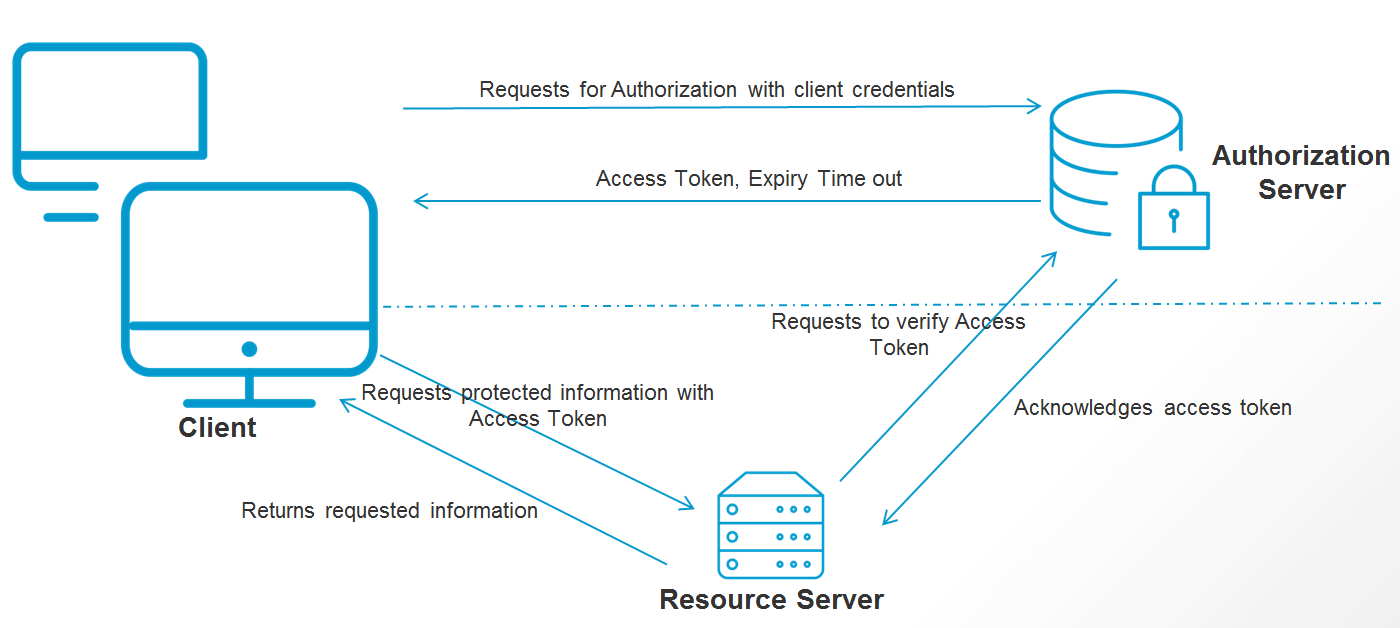
\includegraphics[width=0.8\textwidth]{BAB_TESIS/IMAGES/m2m_auth.png}
    \caption{Skema M2M Authentication}
    \label{fig:m2m}
\end{figure}

		\subsection{Metode Autentikasi Mesin ke Mesin}
		\label{metode autentikasi mesin ke mesin}
		Salah satu metode autentikasi Machine-to-Machine (M2M) menggunakan token merujuk pada proses verifikasi identitas antara dua atau lebih perangkat atau sistem tanpa intervensi manusia. Dalam skenario ini, token digunakan sebagai kredensial atau kunci otentikasi yang diberikan kepada perangkat atau sistem untuk membuktikan identitasnya kepada sistem yang lain.


			\subsubsection{\textit{Basic Access Authentication}}
			\label{basic access authentication}
			\input{BAB_TESIS/BAB3/3_3_1_BASIC_ACCESS_AUTHENTICATION}

			\subsubsection{\textit{Token}}
			\label{token}
			Klien membuat permintaan ke server otorisasi dengan mengirimkan ID klien, rahasia klien, bersama dengan audiens dan klaim-klaim lainnya. Server otorisasi memvalidasi permintaan tersebut, dan, jika berhasil, mengirimkan respons dengan token akses. Klien sekarang dapat menggunakan token akses untuk meminta sumber daya yang dilindungi dari server sumber daya.
Karena klien harus selalu menjaga rahasia klien, pemberian ini hanya dimaksudkan untuk digunakan pada klien terpercaya. Dengan kata lain, klien yang menyimpan rahasia klien harus selalu digunakan di tempat di mana tidak ada risiko rahasia tersebut disalahgunakan. Sebagai contoh, meskipun mungkin ide yang baik untuk menggunakan hibah kredensial klien di sistem internal yang mengirimkan laporan di seluruh web ke bagian lain dari sistem Anda, namun tidak dapat digunakan untuk alat publik yang dapat diakses oleh pengguna eksternal mana pun.
Berikut ini adalah permintaan HTTP yang relevan pada Tabel \ref{tab:req_http} berikut:

\begin{table}[H]
    \caption{Permintaan HTTP}
    \vspace{0.5em}
    \centering
    \begin{tabular}{|c|c|c|}
        \hline
        Permintaan & Deskripsi \\
        \hline \hline
        POST & Metode HTTP \\
        \hline
        /token & Endpoint \\
        \hline
        grant\_type=client\_credentials & Jenis hibah \\
        \hline
        & ID klien \\
        \hline
        & Rahasia klien \\
        \hline
        & Audiens \\
        \hline
    \end{tabular}
    \label{tab:req_http}
\end{table}

Sedangkan berikut contoh respon HTTP yang relevan pada Tabel \ref{tab:res_http} berikut:

\begin{table}[h]
    \caption{Respon HTTP}
    \vspace{0.5em}
    \centering
    \begin{tabular}{|c|c|c|}
        \hline
        Respon & Deskripsi \\
        \hline \hline
        200 OK & Kode status HTTP \\
        \hline
        Content-Type: application/json & Header HTTP \\
        \hline
        Cache-Control: no-store & Header HTTP \\
        \hline
        Pragma: no-cache & Header HTTP \\
        \hline
        \{ & Body \\
        \hline
        "access\_token": "2YotnFZFE & \\
        \hline
        "token\_type": "example", & \\
        \hline
        "expires\_in": 3600, & \\
        \hline
        "example\_parameter": "example\_value" & \\
        \hline
        \} & \\
        \hline
    \end{tabular}
    \label{tab:res_http}
\end{table}

	\section{\textit{Risk-Based Authentication}}
	\label{risk-based authentication}

	\section{\textit{Classification and Regression Tree (CART)}}
	\label{classification and regression tree}

		\subsection{\textit{Random Forest}}
		\label{random forest}


		\subsection{Laju Galat klasifikasi}
		\label{laju galat klasifikasi}

		\subsection{\textit{Variable Importance Measure(VIM)}}
		\label{variable importance measure}


	

%-----------------------------------------------------------------
% Akhir BAB 3
%-----------------------------------------------------------------


%-----------------------------------------------------------------
% Awal BAB 4
%-----------------------------------------------------------------
\chapter{ANALISIS DAN PERANCANGAN SISTEM}
\label{ANALISIS DAN PERANCANGAN SISTEM}

	\section{Deskripsi Umum Sistem}
	\label{rancangan deskripsi umum sistem}
	Analisis sistem terdiri dari gambaran umum sistem yang dapat dilihat pada Gambar \ref{fig:gambaran-umum}, deskripsi sistem, dan diagram alir sistem. Gambaran umum sistem menjelaskan secara singkat tentang sistem yang akan dibangun. Deskripsi sistem menjelaskan tentang sistem yang akan dibangun secara rinci. Diagram alir sistem menjelaskan tentang alur kerja sistem yang akan dibangun.

\begin{figure}[H]
    \centering
    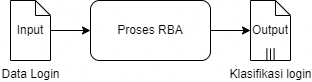
\includegraphics[width=0.6\textwidth]{BAB_TESIS/IMAGES/gambaran-umum.png}
    \caption{Gambaran Umum Sistem}
    \label{fig:gambaran-umum}
\end{figure}



	\section{Analisis Kebutuhan Sistem}
	\label{rancangan analisis kebutuhan sistem}
	Dalam membangun sistem ini, diperlukan analisa kebutuhan fungsional. Kebutuhan fungsional adalah kebutuhan yang berkaitan dengan fungsi-fungsi
yang harus ada dalam sistem. Serta akan dijelaskan kebutuhan perangkat keras dan perangkat lunak yang dibutuhkan dalam membangun sistem ini.

	\section{Pembuatan Sistem}
	\label{rancangan pembuatan sistem}

		\subsection{Pembuatan Sistem Pengenalan Entitas Bernama}
		\label{rancangan pembuatan sistem pengenalan entitas bernama}
		\input{BAB_TESIS/BAB4/3_2_SISTEM_PENGENALAN_ENTITAS_BERNAMA}

		\subsection{Pembuatan Sistem Ekstraksi Kalimat Pernyataan}
		\label{rancangan sistem ekstraksi kalimat pernyataan}
		\input{BAB_TESIS/BAB4/3_3_SISTEM_EKSTRAKSI_KALIMAT_PERNYATAAN}

	\section{Rancangan Antarmuka}
	\label{rancangan antarmuka}

		\subsection{Deskripsi}
		\label{rancangan deskripsi antarmuka}
		\input{BAB_TESIS/BAB4/4_1_DESKRIPSI_RANCANGAN_ANTARMUKA}

		\subsection{\textit{Wireframe}}
	    \label{rancangan wireframe antarmuka}
	    \input{BAB_TESIS/BAB4/4_2_WIREFRAME_ANTARMUKA}

%-----------------------------------------------------------------
% Akhir BAB 4
%-----------------------------------------------------------------


%-----------------------------------------------------------------
% Awal BAB 5
%-----------------------------------------------------------------
\chapter{IMPLEMENTASI SISTEM}
\label{IMPLEMENTASI SISTEM}

	\section{Spesifikasi}
	\label{implementasi spesifikasi}
	\input{BAB_TESIS/BAB5/1_SPESIFIKASI}

	\section{Implementasi Sistem Pengenalan Entitas Bernama}
	\label{implementasi sistem ner}
	\input{BAB_TESIS/BAB5/2_1_IMPLEMENTASI_SISTEM_NER}

	\section{Implementasi Sistem Ekstraksi Kalimat Pernyataan}
	\label{implementasi sistem ekstraksi kalimat pernyataan}
	\input{BAB_TESIS/BAB5/2_2_IMPLEMENTASI_SISTEM_EKTRAKSI_KALIMAT_PERNYATAAN}

%-----------------------------------------------------------------
% Akhir BAB 5
%-----------------------------------------------------------------



%-----------------------------------------------------------------
% Awal BAB 6
%-----------------------------------------------------------------
\chapter{PENGUJIAN DAN PEMBAHASAN SISTEM}
\label{PENGUJIAN DAN PEMBAHASAN SISTEM}
\input{BAB_TESIS/BAB6/1_PENDAHULUAN}

	\section{Pengujian Sistem Pengenalan Entitas Bernama}
	\label{pengujian sistem ner}
	\input{BAB_TESIS/BAB6/2_PENGUJIAN_SISTEM_NER}

	\section{Pengujian Sistem Ekstraksi Kalimat Pernyataan}
	\label{pengujian sistem ekstraksi kalimat pernyataan}
	\input{BAB_TESIS/BAB6/3_PENGUJIAN_SISTEM_EKSTRAKSI_KALIMAT_PERNYATAAN}

%-----------------------------------------------------------------
% Akhir BAB 6
%-----------------------------------------------------------------


%-----------------------------------------------------------------
% Awal BAB 7
%-----------------------------------------------------------------
\chapter{PENUTUP}
\label{PENUTUP}

	\section{Kesimpulan}
	\label{penutup kesimpulan}
	Kesimpulan dari penelitian ini adalah sebagai berikut:
\begin{enumerate}
	\item Model yang dihasilkan belum dapat mengklasifikasi risiko autentikasi dengan baik. Sistem autentikasi M2M berbasis risiko menggunakan Random Forest dapat mengklasikasi risiko autentikasi. Dengan akurasi 70.8\%, presisi 70.1\%, \textit{recall} 96.8\%, dan \textit{F1-score} 71.3\%. Ketimpangan akurasi dan \textit{recall} disebabkan oleh ketidakseimbangan jumlah data pada kelas yang berbeda.
	\item Pembatasan fitur kepentingan dapat berpengaruh pada akurasi sistem.
\end{enumerate}


	\section{Saran}
	\label{penutup saran}
	Penelitian ini masih memiliki beberapa kekurangan yang dapat diperbaiki pada penelitian selanjutnya, yaitu:
\begin{enumerate}
	\item Penelitian ini masih menggunakan dataset hybrid. Sehingga perlu dilakukan penelitian lebih lanjut dengan menggunakan dataset asli.
	\item Akurasi sistem masih dapat ditingkatkan, serta perlu dilakukan penelitian lebih lanjut untuk meningkatkan keamanan sistem.
	\item Opitimasi parameter Random Forest masih dapat dilakukan lebih lanjut.
	\item Dapat dilakukan perbandingan dengan memilih target parameter yang berbeda.
\end{enumerate}


%-----------------------------------------------------------------
% Akhir BAB 7
%-----------------------------------------------------------------

%-----------------------------------------------------------------
% Awal Daftar Pustaka
%-----------------------------------------------------------------
\begin{thebibliography}{99}
    \addcontentsline{toc}{chapter}{DAFTAR PUSTAKA}
    
    \bibitem[Agarwal et al.(2016)]{Agarwal2016}
    Agarwal, L., Khan, H., \& Hengartner, U. (2016). Ask Me Again But Don’t Annoy Me: Evaluating Re-authentication Strategies for Smartphones. 221–236. \url{https://www.usenix.org/conference/soups2016/technical-sessions/presentation/agarwal}
    
    \bibitem[Alam \& Vuong(2013)]{Alam2013}
    Alam, M. S., \& Vuong, S. T. (2013). Random Forest Classification for Detecting Android Malware. 2013 IEEE International Conference on Green Computing and Communications and IEEE Internet of Things and IEEE Cyber, Physical and Social Computing, 663–669. \url{https://doi.org/10.1109/greencom-ithings-cpscom.2013.122}
    
    \bibitem[Cabarcos et al.(2019)]{Cabarcos2019}
    Cabarcos, P. A., Arias-Cabarcos, P., Krupitzer, C., \& Becker, C. (2019). A Survey on Adaptive Authentication. ACM Computing Surveys, 52(4), 80. \url{https://doi.org/10.1145/3336117}
    
    \bibitem[Doerfler et al.(2019)]{Doerfler2019}
    Doerfler, P., Thomas, K., Marincenko, M., Ranieri, J., Jiang, Y., Moscicki, A., \& McCoy, D. (2019). Evaluating Login Challenges as a Defense Against Account Takeover. 372–382. \url{https://doi.org/10.1145/3308558.3313481}
    
    \bibitem[Dutson et al.(2019)]{Dutson2019}
    Dutson, J., Allen, D., Eggett, D. L., \& Seamons, K. E. (2019). Don’t Punish all of us: Measuring User Attitudes about Two-Factor Authentication. 119–128. \url{https://doi.org/10.1109/eurospw.2019.00020}
    
    \bibitem[Braunstein(2022)]{Braunstein2022}
    Braunstein, Mark L. (2022). FHIR. Computers in Health Care, 233–291. \url{https://doi.org/10.1007/978-3-030-91563-6_9}
    
    \bibitem[Misbahuddin et al.(2017)]{Misbahuddin2017}
    Misbahuddin, M., B. S. Bindhumadhava, B. S. Bindhumadhava, Bindhumadhava, B. S., \& Dheeptha, B. (2017). Design of a risk-based authentication system using machine learning techniques. 1–6. \url{https://doi.org/10.1109/uic-atc.2017.8397628}
    
    \bibitem[Prasad et al.(2017)]{Prasad2017}
    Prasad, K. K., K, K. P., \& Aithal, S. (2017). A Study on Enhancing Mobile Banking Services Using Location Based Authentication. \url{https://doi.org/10.47992/ijmts.2581.6012.0006}
    
    \bibitem[Rahat et al.(2021)]{Rahat2021}
    Rahat, Tamjid Al, Feng, Yu, \& Tian, Yuan. (2021). Cerberus. Cornell University - ArXiv. \url{https://doi.org/10.1145/3548606.3559381}
    
    \bibitem[Roy \& Dasgupta(2018)]{Roy2018}
    Roy, A., \& Dasgupta, D. (2018). A fuzzy decision support system for multifactor authentication. Soft Computing - A Fusion of Foundations, Methodologies and Applications, 22(12), 3959–3981. \url{https://doi.org/10.1007/s00500-017-2607-6}
    
    \bibitem[Solapurkar(2016)]{Solapurkar2016}
    Solapurkar, P. (2016). Building secure healthcare services using OAuth 2.0 and JSON web token in IOT cloud scenario. International Conferences on Contemporary Computing and Informatics, 99–104. \url{https://doi.org/10.1109/ic3i.2016.7917942}
    
    \bibitem[Speiser et al.(2019)]{Speiser2019}
    Speiser, J. L., Miller, M., Miller, M. E., Tooze, J. A., \& Ip, E. H. (2019). A Comparison of Random Forest Variable Selection Methods for Classification Prediction Modeling. Expert Systems With Applications, 134, 93–101. \url{https://doi.org/10.1016/j.eswa.2019.05.028}
    
    \bibitem[Wiefling et al.(2021)]{Wiefling2021}
    Wiefling, Stephan, Markus Dürmuth, \& Luigi Lo Iacono. (2021). What’s in Score for Website Users: A Data-driven Long-term Study on Risk-based Authentication Characteristics. Financial Cryptography. \url{https://doi.org/10.1007/978-3-662-64331-0_19}
    
    \bibitem[Wiefling et al.(2022)]{Wiefling2022}
    Wiefling, Stephan, Paul René Jørgensen, Sigurd Thunem, \& Luigi Lo Iacono. (2022). Pump Up Password Security! Evaluating and Enhancing Risk-Based Authentication on a Real-World Large-Scale Online Service. ACM Transactions on Privacy and Security. \url{https://doi.org/10.1145/3546069}
    
    \bibitem[Taneja(2013)]{Taneja2013}
    Taneja, M. (2013). An analytics framework to detect compromised IoT devices using mobility behavior. Information and Communication Technology Convergence, 38–43. \url{https://doi.org/10.1109/ictc.2013.6675302}
    
    \bibitem[Thomas et al.(2017)]{Thomas2017}
    Thomas, K., Li, F., Zand, A., Barrett, J., Ranieri, J., Invernizzi, L., Markov, Y., Comanescu, O., Eranti, V., Moscicki, A., Margolis, D., Paxson, V., \& Bursztein, E. (2017). Data Breaches, Phishing, or Malware?: Understanding the Risks of Stolen Credentials. 1421–1434. \url{https://doi.org/10.1145/3133956.3134067}
    
    \bibitem[Zhang et al.(2012)]{Zhang2012}
    Zhang, F., Kondoro, A., \& Muftic, S. (2012). Location-Based Authentication and Authorization Using Smart Phones. 2012 IEEE 11th International Conference on Trust, Security and Privacy in Computing and Communications, 1285–1292. \url{https://doi.org/10.1109/trustcom.2012.198}
\end{thebibliography}

%-----------------------------------------------------------------
% Akhir Daftar Pustaka
%-----------------------------------------------------------------


%-----------------------------------------------------------------
% Awal lampiran
%-----------------------------------------------------------------
\appendix

\chapter{BERKAS JSON UNTUK MODEL SISTEM PENGENALAN ENTITAS BERNAMA}
\label{BERKAS JSON UNTUK MODEL SISTEM PENGENALAN ENTITAS BERNAMA}
\input{BAB_TESIS/BAB9_LAMPIRAN/1_BERKAS_MODEL_NER}

%-----------------------------------------------------------------
% Akhir lampiran
%-----------------------------------------------------------------

\end{document}